%!TEX program=luatex

\newpage
\section{Introduction}
Les systèmes de recommandation demeurent aujourd'hui un moyen non négligeable pour l'amélioration de l’expérience utilisateur sur les réseaux sociaux, le e-commerce et sur les moteurs de recherche.\\
Ils contribuent d'une manière considérable dans l'accroissement de plusieurs entreprises technologiques tels que \emph{Facebook}, \emph{Amazon} ou \emph{Google} qui exploitent des quantités massives de données (Big data) afin de faire des recommandations avec un niveau de confiance assez élevé.\\
Il sera question dans ce chapitre d’effectuer une description de l'état de l'art par la présentation des systèmes de recommandations et leurs utilisations pour la prédiction des comportements des utilisateurs, une brève présentation de l'apprentissage automatique et ses différentes techniques, et nous allons conclure par l'introduction des techniques de profilage d'utilisateurs.

\section{Apprentissage automatique}
    \subsection{Définition}
    \emph{L'apprentissage automatique} comme il a été défini par \emph{svensson} et \emph{Söderberg} dans leur article «Machines that learn»\cite{svensson} désigne la conception et le développement d'algorithmes et de techniques qui permettent aux ordinateurs d'apprendre et de prédire de façon intelligente.\\
    Souvent on a recours à l'apprentissage automatique lorsque on ignore le modèle adéquat à utiliser pour la résolution d'un problème donné, on peut citer aussi :
    \begin{itemize}
        \item Le manque d'expertise sur le problème.
        \item La difficulté et la complexité des solutions disponibles. 
        \item L'espace des solutions du problème est très grand et change dans le temps. 
    \end{itemize}
    L'apprentissage automatique est utilisé dans différents domaines: économie, divertissement et multimédia.

    \subsection{Le processus d'apprentissage}
    Afin d'implémenter un modèle performant et précis, certains pré-traitements doivent être fait comme le précise Han dans son livre «DATA MINING Concepts»\cite{Han}, on retrouve:

    \begin{itemize}
    	\item Collecte des données : le but de cette étape est de récupérer les données représentatives et qui ont un sens par rapport au problème traité.
    	\item Séléction des caractéristiques (Features) : c'est l'étape la plus importante de ce processus, la performance du modèle finale y dépend.
    	\item Nettoyage de données : suppression des données aberrantes et remplacement des valeurs manquantes, normalisation et discrétisation.
    	\item Choix du type d'apprentissage selon le problème posé.
    	\item Apprentissage.
    	\item Évaluation : Évaluer les capacités prédictives du modèle et sa généralisation, et comparer ces performances par rapport a d'autres techniques.
    \end{itemize}

    \subsection{Paradigmes de l'apprentissage automatique}
    Nous avons évoqué précédemment le type d'apprentissage a choisir dans le processus d'apprentissage, on peut trouver plusieurs algorithmes d'apprentissage automatique.\\
    Ces algorithmes peuvent être classés dans deux groupes basés sur la façon avec laquelle ils \emph{apprennent} à prédire : supervisé, non supervisé et par renforcement.

        \subsubsection{Apprentissage automatique supervisé}
        L'apprentissage supervisé est ainsi nommé car il nécessite l'intervention de l'être humain (souvent un expert) pour spécifier à l'algorithme les résultats qu'il devrait fournir.\\
        L'apprentissage supervisé nécessite que les sorties possibles de l'algorithme soient déjà connues et que les données utilisées pour former l'algorithme soient déjà étiquetées avec des réponses correctes. Donc, les données d'apprentissage doivent être labellisées/classifiées au préalable en plus des caractéristique d'identification.\\

        parmi les approches utilisées pour l'apprentissage automatique supervisé, on retrouve :

        \textbf{•La régression :} la régression est le problème de l'estimation ou de la prédiction d'une quantité continue. Combien de clients partiront pour un concurrent cette année? 
        ces algorithmes sont :L'analyse de régression fait partie de l'analyse prédictive et exploite la co-relation entre dépendante (cible) et variables indépendantes.\\
        Les modèles de régression notables sont: régression linéaire, régression logistique, pas à pas
        Régression, régression des moindres carrés ordinaires (OLSR), splines de régression adaptative multivariée (MARS), localement Lissage de nuage de points estimé (LOESS).\cite{surveymachinelearningregression}

        \textbf{•Classification:}
        La classification consiste à attribuer des observations à des catégories discrètes plutôt qu'à estimer des quantités continues exemple : Un client donné nous quittera-t-il pour un concurrent? Est-ce qu'un patient donné à un cancer?\\
        Les algorithmes pour effectuer la classification sont :

        - Algorithmes d'arbre de décision: Un arbre de décision construit une structure de type arbre de solutions possibles à un problème basé sur certaines contraintes.\\ 
        Il est ainsi nommé car il commence par une simple décision simple ou racine, qui se décompose ensuite en un certain nombre de branches jusqu'à ce qu'une décision ou une prédiction soit faite, formant un arbre.\\
        Ils sont favorisés pour sa capacité à formaliser le problème dans le processus de la main qui à son tour aide à identifier le potentiel solutions plus rapides et plus précises que d'autres. Exemples: Arbre de classification et de régression (CART), itératif Dichotomiseur 3 (ID3), C4.5 et C5.0, détection automatique d'interférence au chi carré (CHAID), souche de décision, M5, Arbres décisionnels conditionnels, etc.\cite{surveymachinelearningclassification}

        - Algorithmes bayésiens: Un groupe d'algorithmes ML utilise le théorème de Bayes pour résoudre les problèmes de classification et de régression.\\
        Exemples: Bayes naïves, bayes naïves gaussiennes, bayes naïves multinomiales, estimateurs à une dépendance en moyenne (AODE), Bayesian Belief Network (BBN), réseau bayésien (BN) etc.\cite{surveymachinelearningclassification}

        - Machine de vecteur de soutien (SVM): SVM est une technique ML si populaire qu'elle peut être un groupe à part entière. Utilise un hyperplan séparateur ou une décision Les limites de décision de plan todemarcate parmi un ensemble de points de données sont classées avec des étiquettes différentes.\\ 
        C'est strictement algorithme de classification supervisé. En d'autres termes, l'algorithme développe un hyperplan optimal en utilisant des données d'entrée ou données de formation et ce plan de décision à tour de rôle de nouveaux exemples.\\ 
        Basé sur le noyau utilisé, SVM peut effectuer classification linéaire et non linéaire.\cite{surveymachinelearningclassification}


        \subsubsection{Apprentissage automatique non-supervisé}
        L'apprentissage automatique non supervisé consiste à déduire une fonction à partir de données \textbf{non labellisées/étiquetées} en utilisant des algorithmes basés sur le calcul de la similarité entre ces données.\\
        Les données seront divisé en sous-groupes de manière que ces derniers seront le plus possible similaires.
        Ce type d'apprentissage est très utilisé dans le domaine de l'imagerie médical et la détection d'anomalie.\\
        La technique la plus utilisée est \textbf{le clustering}, la mise en cluster concerne l'utilisation d'un modèle intégré dans les ensembles de données pour classer et étiqueter les données en conséquence.\\
        Exemples: K-Means, K-Medians, Propagation d'Affinité, Clustering Spectral, Cluster hiérarchique Ward, Clustering agglomératif. DBSCAN, mélanges gaussiens, bouleau, décalage moyen, maximisation des attentes (EM), ...etc.\cite{surveymachinelearningclustering}

        \subsubsection{Apprentissage automatique par renforcement}
        Un type plus récent de problème d'apprentissage qui a acquis beaucoup de traction récemment s'appelle l'apprentissage par renforcement.\\ 
        Dans ce type d'apprentissage, aucun exemple n'est fourni a la machine sauf une information sous la forme d'un signal de récompense.\\ 
        Les méthodes d'apprentissage par renforcement ressemblent à la façon dont les humains apprennent: la machine essaie un tas de choses différentes et est récompensée quand elle fait quelque chose de bien.\\
        L'apprentissage par renforcement est utile dans les cas où l'espace de solution est énorme ou infini et s'applique généralement dans les cas où la machine peut être considérée comme un agent interagissant avec son environnement (Agent cognitif).


\section{Les systèmes de recommandations}
Un nombre croissant d'entreprises en ligne utilisent des systèmes de recommandation pour accroître l'interaction de l'utilisateur et enrichir le potentiel d'achat. Les cas d'utilisation des systèmes de recommandation ont connu une expansion rapide dans de nombreux aspects du commerce électronique et des médias en ligne au cours des cinq dernières années, et nous prévoyons que cette tendance se poursuivra.\\ 
Les systèmes de recommandation (souvent appelés «moteurs de recommandation») peuvent modifier la façon dont les sites Web communiquent avec les utilisateurs et permettre aux entreprises de maximiser leur retour sur investissement en fonction des informations qu'ils peuvent recueillir sur les préférences et les achats de chaque client.
    \subsection{Définition}
    Un système de recommandation est un mécanisme de filtrage de l'information qui permet de proposer à des utilisateurs des éléments qui sont susceptibles de les intéresser selon leurs préférences et leurs comportements.\\
    Le but final est de prédire leur appréciation afin de leur suggérer des éléments similaires qu'ils seraient en mesure d'apprécier.\\
    Ces systèmes utilisent des techniques très avancés de l'intelligence artificielle tels que l'apprentissage automatique, le traitement automatique de la langue et la recherche d'informations. 

    \subsection{Quelques exemples des systèmes de recommandations}
    Compte tenu de l'importance des systèmes de recommandation qui permettent de cibler l'utilisateur selon ses caractéristiques (profil), plusieurs modèle de ces derniers ont vue le jour. Nous allons expliciter quelques uns :

        \subsubsection*{Système de recommandation pour les réseaux sociaux :}
        \textbf{LinkedIn :} LinkedIn est un réseau social professionnel qui fait usage des systèmes de recommandation.Il utilise un filtrage collaboratif à base d'objets (Membres, Sociétés, Groupes) grâce à un module de recommandation disponible dans chaque profil permettant de recommander d'autres membres fréquemment associés au profil actuel ou du même groupe ou postulant au même emploi.\\
            \begin{figure}[H]
                \centering
                   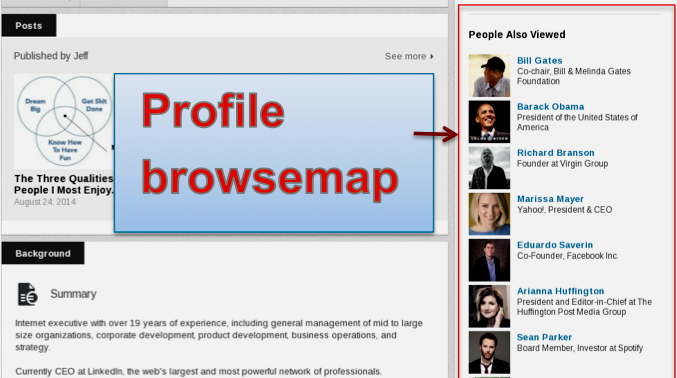
\includegraphics[height=180pt,width=350pt]{img/chapter1/linkedin.png}
                \caption{Recommandations sur le réseau social LinkedIn.}
            \end{figure}

        \textbf{Facebook :} Facebook est un réseau social en ligne qui permet aux 829 millions d’utilisateurs quotidien \cite{userFacebook} d'interagir avec d'autres personnes (et marques) autour du monde en partageant et en taggant des photos, en publiant des liens, en créant des groupes et des événements, en commentant et en chattant. Afin de recommander des amis, des groupes, des pages ou bien des événements, Facebook utilise plusieurs types de systèmes de recommandation tel que le filtrage collaboratif et le filtrage basé contenu.\\ 

        \subsubsection*{Système de recommandation pour les Plateformes de e-commerce :}
        \textbf{Amazon :} Amazon est un site internet de vente en ligne, très répandu dans le monde. Il compte selon \cite{refamazonus} 300 millions de comptes utilisateurs. Pour cela, le développement d'un système de recommandation était une tache majeure. Les ingénieurs d'Amazon ont opté depuis le début pour une approche basée sur un \emph{filtrage collaboratif basé mémoire} (memory-based collaborative filtering) qui permet de recommander les produits en se basant sur les produits préférés par les utilisateurs similaires mais aussi de cibler les produits similaires à ceux déjà achetés ou notés\cite{amazon}. Cette approche a été essentielle a Amazon puisque’elle représente à elle seule 35\% du chiffre d'affaires d'Amazon selon une étude de McKinsey's Chicago office \cite{McKinsey}.\\ 
            \begin{figure}[H]
                \centering
                   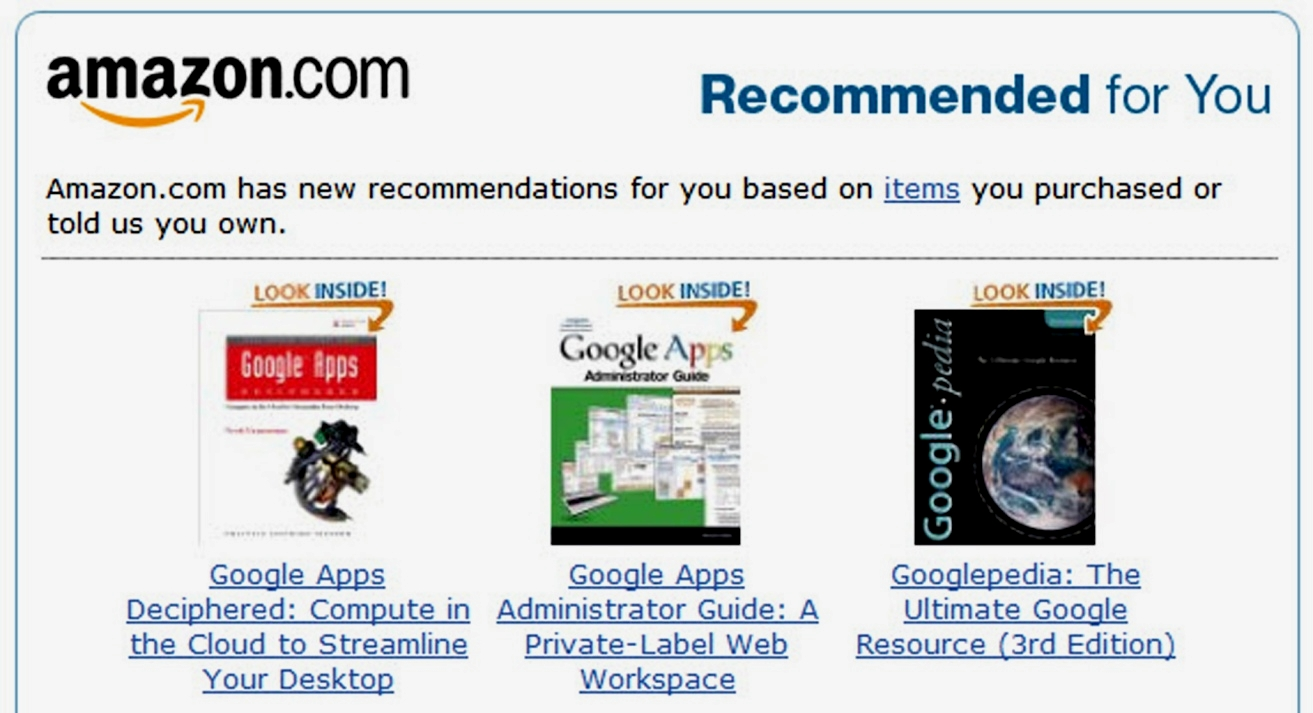
\includegraphics[height=180pt,width=350pt]{img/chapter1/amazon.jpg}
                \caption{Recommandations sur le site \emph{amazon.com}}
            \end{figure}

        \subsubsection*{Système de recommandation pour les plate-forme de streaming vidéo :}
        \textbf{Netflix :} Netflix est un média qui propose du contenu vidéo (films, séries, documentaires...) en flux continu sur internet. Comme ce site est très prisé partout dans le monde, Netflix se concentre beaucoup sur les systèmes de recommandation pour proposer les vidéos appropriées aux utilisateurs. Parmi les méthodes utilisées, on retrouve :
            \begin{enumerate}
                \item \textbf{Top-N VideoRanker :} C'est un algorithme permettant de retrouver les meilleures recommandations personnalisée pour chaque abonné en se basant sur le classement du nombre de vues des films, les tendances et la popularité.\\

                \item \textbf{Personnalized VideoRanker :} C'est un algorithme personnalisé qui se base sur le profil de l'utilisateur pour le classement de vidéo populaires. La précision amené par cet algorithme été nettement plus intéressante que l'algorithme précédent \cite{netflix} .\\

                \item \textbf{Tendances du moment :} Cet algorithme propose les tendances du moment combinés au profil utilisateur. Les tendances restent aussi un puissant moyen de prédiction.\\

                \item \textbf{Continuité :} C'est une solution qui propose un contenu vidéo qui est dans la continuité du contenu actuel comme le prochain épisode d'une série.\\

                \item \textbf{Filtrage par similarité entre vidéos :} C'est une solution permettant de prédire des vidéos de la même catégorie que la vidéo actuelle.\\

                \item \textbf{Génération des pages :} À la création du site, Netflix proposait de petites fenêtres sur les pages générées. Celles-ci représentaient les catégories et les genres des Films ou séries. À partir de 2015, les systèmes de recommandations ont rendu la génération des pages beaucoup plus personnalisés ce qui fait que certaines fenêtres inutiles ont disparu.\\

                \item \textbf{Évidence :} Cet algorithme recommande des films a l'utilisateur en utilisant certaines caractéristiques des films (acteurs fameux, oscars...).\cite{netflix}\\
            \end{enumerate}
            \begin{figure}[H]
                \centering
                   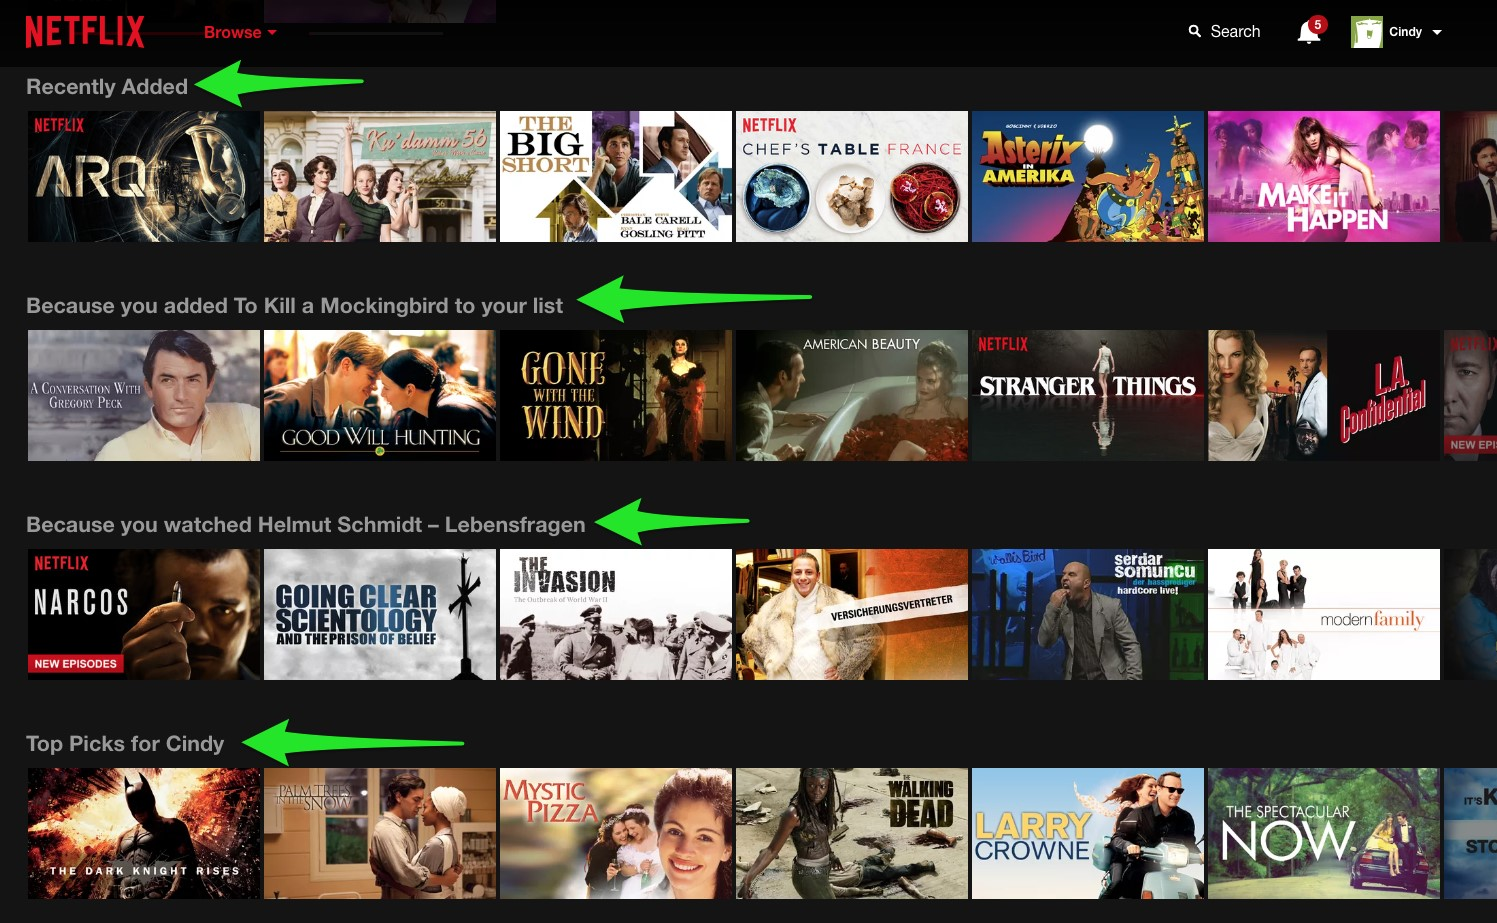
\includegraphics[height=180pt,width=350pt]{img/chapter1/netflix.jpg}
                \caption{Recommandations sur la plate-forme Netflix}
            \end{figure}

        \subsubsection*{Système de recommandation pour les articles de presse :} 
        \textbf{Google News :} c'est une plate-forme en ligne d'articles de presse obtenue de différentes sources. Initialement Google utilisait un filtrage collaboratif, ensuite ils ont combiné l'approche collaboratif et l'approche basée contenu pour offrir de meilleurs résultats.\cite{gglnews}

        \textbf{Buzzer :} c'est un système de recommandation développé par l'université de Dublin sur la base de nombre de clics limités sur des pages de presse en ligne. Ce laboratoire a testé des approches basées sur le public (\emph{rank}, \emph{friends rank} et \emph{content rank}). L'évaluation a permis de constater que le nombre de clics le plus important était généré par le \textbf{friends rank} a continuer .... c'est a dire friends rank.\cite{gglnews}\\
            \begin{figure}[H]
                \centering
                   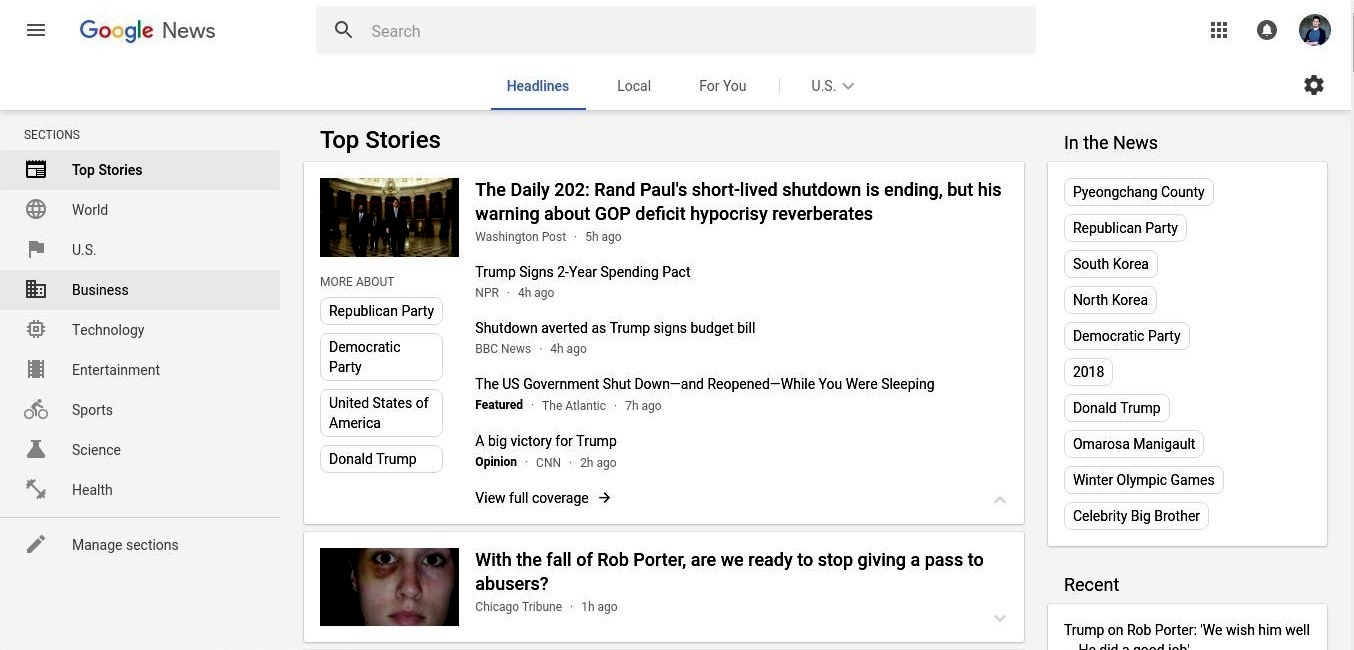
\includegraphics[height=180pt,width=350pt]{img/chapter1/news.jpg}
                \caption{Portail de GoogleNews avec des recommandations}
            \end{figure}

        Au terme de ce tour d'horizon, on constate que les systèmes de recommandations participent grandement à promouvoir les objets (produits, multimédia, articles de presse...) puisqu'ils représentent 80\% du contenu proposé. Ceci a diminué des activités des moteurs de recherche de chaque site décrit précédemment puisqu'elles représentent que 20\% des données proposées selon un article intitulé "The Netflix Recommender System:Algorithms,Business Value,and Innovation" apparu sur le site officiel de Netflix. \cite{netflix}\\

    \subsection{Types de systèmes de recommandations}
    définition en 1 ligne ou 2.
    \begin{figure}[H]
            \centering
               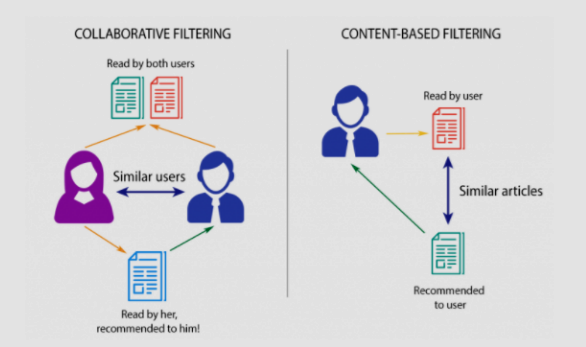
\includegraphics[height=180pt,width=350pt]{img/chapter1/filtering.png}
            \caption{Types de systèmes de recommandations\cite{figfiltering}}

    \end{figure}

    \begin{itemize}
        \item \textbf{Filtrage basé contenu (Content-based filtering) :\\}
        C'est une des méthodes de recommandation les plus simples; elle consiste à recommander les items ayant le plus de similarité avec les préférences de l'utilisateur.\\

        \item \textbf{Filtrage collaboratif (Collaborative filtering) :\\}
        Dans cette approche, la recommandation se fait en utilisant les préférences des profils jugés similaires au profil ciblé, et cela grâce aux préférences précédentes des personnes qui sont regrouper dans des structures de données permettant de calculer la similarité. Parmi les méthodes utilisées on retrouve :
            \begin{enumerate}
                \item \textbf{Filtrage collaboratif basé mémoire (Memory-based collaborative filtering) : }Les notes d'appréciation des utilisateurs sont utilisées pour le calcul de similarité entre utilisateurs ou entre les objets afin de permettre de cibler au mieux les préférences.\\
                \item \textbf{Filtrage collaboratif basé model (Model-based collaborative filtering) : }Cette technique utilise un modèle de prédiction propre à chaque utilisateur selon les techniques de DataMining, de Recherche d'Informations et de Traitement Automatique du Langage.\\
            \end{enumerate}

        \item \textbf{Filtrage hybride (Hybrid recommender system) :\\}
        Cette approche utilise filtrage basé contenu et le filtrage collaboratif pour faire face aux problèmes rencontrés en utilisant un filtrage basé contenu seul ou en utilisant un filtrage collaboratif seul. Le but est d'avoir une précision maximale c'est a dire de meilleurs capacités de prédiction.\cite{filtering}
    \end{itemize}

    \subsection*{Avantages des systèmes de recommandations}
    L'utilisation des systèmes de recommandations est une approche gagnante sur tout les fronts que ce soit pour un utilisateur qui trouve tout ce qu'il cherche de manière facile ou pour l'organisme qui désire générer des gains économiques rapidement et efficacement.\\
    En effet, les recommandations ciblent directement un article précis pour un utilisateur précis, ce qui va pousser ce dernier à s'accrocher et à continuer sa recherche afin de trouver la meilleure offre possible. D'un autre coté, l'utilisation des profils utilisateurs dans les systèmes de recommandations les rendent beaucoup plus personnalisés et conformes aux besoins réels de l'utilisateur.\cite{figfiltering}

\section{Systèmes de recommandations pour les articles de presse}
    \subsection*{Contraintes liées a la recommandation des articles de presse}
    L'utilisation des systèmes de recommandation pour des sites de vente en ligne ou des réseaux sociaux est très différente de son utilisation pour une revue de presse personnalisée, puisqu'ils y existent des contraintes spécifiques aux revues de presse.
    Parmi ces contraintes on retrouve :
    \begin{itemize}
        \item \textbf{Le démarrage à froid (Cold start) : \label{froid}}c'est à dire on ne possède aucune information précédente sur l'utilisateur, ses caractéristiques ou son profil. Généralement c'est lors d'une navigation sans identification que ce cas se présente.\\
        \item \textbf{Le manque de données (Data sparsity) : }les structures de données liées au profil de l'utilisateur peuvent être vides ou très denses ce qui nécessite pour les deux cas un traitement particulier.\\
        \item \textbf{La récence (recency) : \label{recence}}dans un système de recommandation traitant des articles de presse, il est inconcevable de proposer d'anciens articles puisque leur importance diminue avec le temps et l'application deviendrait une simple fenêtre à articles ce qui est contraire aux exigences des systèmes de recommandation de proposer des articles en temps-réel.\\
        \item \textbf{Les Changements des intérêts des utilisateurs : }c'est la capacité d'adaptation du système de recommandation aux besoins de l'utilisateur, c'est à dire que si les tendances de ce dernier changent le système doit proposer des articles adaptés à ses nouvelles tendances.\\
        \item \textbf{L'évolutivité (scalability) : }C'est la capacité du système à servir plusieurs utilisateurs à la fois et sa rapidité d'interaction avec la source des articles. La dynamique de l'environnement exige une rapidité de calcul en temps réel.\\ 
    \end{itemize}

    \subsection{État de l'art des systèmes de recommandations pour les News}
    De nombreux cadres ont été développés pour la recommandation des articles de presse au cours des dernières années. Certains d'entre eux ont utilisé le filtrage basé sur le contenu; d'autres ce sont basés sur un filtrage collaboratif ou une combinaison de deux techniques de recommandation résultant en une approche hybride pour générer des recommandations d'articles de presse pour les utilisateurs.\\

    Parmi les travaux de recherche dans le domaine des articles de presse, \emph{Sood} et \emph{Kaur}\cite{surveyrecommender1} explicitent dans leur enquête sur les systèmes de recommandations d'articles de presse quelques uns:

    LOGO\cite{27} intègre les préférences de lecture à long terme et à court terme des utilisateurs lorsqu'ils leur recommandent des informations. Profil à long terme d'un utilisateur est construit sur la base d'un schéma de pondération sensible au temps \cite{28} et le profil à court terme en analysant le dernier historique de lecture de l'utilisateur. Les deux peuvent aider à déterminer les nouvelles recommandations pour les utilisateurs.

    Tan et Tee \cite{29} ont présenté dans leur publication «Learning User Profiles for Personalized Information Dissemination» un système de recommandation personnalisé appelé PIN. PIN récupère et classe les articles d'actualité en fonction du profil de l'utilisateur, qui est initialement défini par l'utilisateur comme une liste de mots clés, puis appris à partir des commentaires des utilisateurs à l'aide de la technologie de réseau neuronal. Lors de l'interaction avec le code confidentiel, les utilisateurs fournissent des commentaires explicites en évaluant les articles.

    Hochul Jeon, Taehwan Kim et Joongmin Choi\cite{30} ont proposé un modèle de récupération d'information personnalisée. Les informations des utilisateurs doivent être extraites pour trouver la similarité entre elles et les informations devraient être recommandées aux utilisateurs par des groupes d'utilisateurs similaires.

    Un navigateur d'articles de presse à usage spécifique pour PDA (Personal Digital Assistant), nommé WebClipping2, est présenté dans l'article publié en 2006 intitulé «Evaluating adaptive user profiles for news classification»\cite{31}. WebClipping2 utilise un classificateur bayésien afin de calculer la probabilité qu'un article spécifique soit jugé intéressant par l'utilisateur. Plutôt que de demander aux utilisateurs de fournir des retours explicites, WebClipping2 observe le temps de lecture total, le nombre de lignes lues et d'autres caractéristiques du comportement de l'utilisateur pour déduire les intérêts de l'utilisateur.

    Le système décrit dans «Adaptive User Profile Model and Collaborative Filtering for Personalized News»\cite{32} par \emph{Wang} se concentre sur le changement des préférences de l'utilisateur. Dans ce système, les intérêts de l'utilisateur sont modélisés par un arbre multicouche avec une structure dynamiquement modifiable, dont les couches supérieures sont utilisées pour modéliser les intérêts des utilisateurs sur des catégories fixes, et les couches inférieures pour les événements dynamiques. Ce modèle peut suivre les comportements de lecture de l'utilisateur sur des catégories fixes et des événements dynamiques, et par conséquent capturer les changements d'intérêt.

    Fikadu Gemechu, Zhang Yu et Liu Ting \cite{34} ont proposé un cadre dans lequel un module de profil utilisateur est incorporé en tant que composant intégral du processus de récupération de l'information afin que les résultats soient filtrés en fonction du profil de l'utilisateur.

    Liang et Lai \cite{35} ont proposé une approche temporelle pour construire des profils d'utilisateurs à partir du comportement de navigation, qui prenait en compte le temps passé par l'utilisateur à lire les articles et les activités récentes de l'utilisateur.

    Lee, Liu et Cho \cite{36} ont dévelopé une méthode appelé «Automatic identification of user goals in Web search» pour apprendre automatiquement l'intérêt des utilisateurs en se basant sur l'historique des clics passés. L'intérêt de l'utilisateur appris est intégré dans le Page Rank sensible pour générer un classement personnalisé.


\section{Profilage d'utilisateur}
Dans un monde où l'utilisation des systèmes de recommandation ne cesse de croître, la personnalisation d'un objet recommandé devient très importante surtout pour les systèmes basés sur les caractéristiques de chaque profil ou les systèmes hybrides.\\
Nous avons jusqu'ici utilisé le terme "profilage" pas très formellement, nous donnons dans ce qui suit une explication plus précise de ce concept.\\ 

    \subsection{Définition}
    Un profilage est une représentation des intérêts de l'utilisateur sous forme d'une structure de données comportant des informations propres à chaque utilisateur (coordonnés, préférences,...etc) qui peuvent être traités par des systèmes d'exploitation, des SGBD ou des moteurs de recherches.

    \subsection{Contenu du profil utilisateur}
    Un profil utilisateur contient des informations qui sont jugées utiles et cela en fonction des besoins.\\
    On retrouve par exemple :\\
    \begin{itemize}
        \item Un historique qui permet de modéliser les comportement des utilisateurs.
        \item Les centres d’intérêts et les préférences relatives au problème à traité afin de construire un modèle de prédiction pour la recommandation.
    \end{itemize}

    \subsection{Types de profilage d'utilisateurs}
        \subsubsection{Profilage explicite (Explicit user profiling)}
        Ce type de profilage se base uniquement sur les informations fournies par l'utilisateur tel une évaluation d'un objet ou un remplissage de formulaire. Cette approche n'est pas entièrement satisfaisante car la méfiance des utilisateurs (non divulgation des coordonnées, données erronées...) rend ce type de profilage très dépassé en fonction des besoins.

        \subsubsection{Profilage implicite (implicit user profiling)}
        Comme l'approche de profilage explicite ne donnaient pas suffisamment de bons résultats, l'approche implicite utilise le comportement de l'utilisateur (clics, temps de parcours, historique...). Certes cette méthode réduit l'erreur dans la prédiction mais présente un certain défaut: par exemple, quand un utilisateur achète un produit sur une plateforme de commerce en ligne pour un ami, cela ne veut en aucun cas dire que l'utilisateur est intéressé par ce produit.

        \subsubsection{Profilage hybride (Hybrid user profiling)}
        Ce type de profilage englobe l'approche explicite, qui permet de récolter des informations à travers des formulaires, et l'approche implicite, qui récupère les comportements de l'utilisateur. Cette méthode de profilage est plus efficace notamment pour l'augmentation des capacités prédictives lors de la recommandation d'informations temporelles (articles de presse).

    \subsection{Extraction de profil utilisateur}
    L'extraction du profil utilisateur représente une étape clé dans le processus de profilage. Elle peut se faire de manière générale par extraction des données (amis, contenu partagé, coordonnées...) à partir des sites web, des réseaux sociaux ou des plateformes de e-commerce. Néanmoins ceci ne suffit pas dans tous les cas, faute de précision du ciblage.\\
    Une autre approche a été introduite pour l'extraction des profils par Yoshinori Hijikata \cite{profil} qui a fait une étude sur l'extraction de profils suivant le mouvement de la souris de l'ordinateur. On peut citer quelques unes des informations qui peuvent être ainsi collectées :
    \begin{itemize}
        \item Suivi de texte: le déplacement du pointeur de la souris le long d'une phrase pendant la lecture.
        \item Pointage de lien: positionnement du pointeur de la souris sur un lien sans forcément cliquer dessus.
        \item Clique sur un lien: en cliquant sur un lien pour passer à une autre page.
        \item Sélection de texte: sélection du texte en faisant glisser le pointeur de la souris.
        \item Défilement: vitesse de défilement d'une fenêtre.
        \item Enregistrement de signets: enregistrement d'une page en tant que signet.
        \item Enregistrement d'une page : enregistrement d'un document HTML.
        \item Impression: impression d'une page.
        \item Déplacement de la fenêtre: déplacement d'une fenêtre du navigateur Web.
        \item Redimensionnement de la fenêtre: modification de la taille de la fenêtre du navigateur Web.
        \item TimeOnMouse: nombre de millisecondes passées par l'utilisateur lors du déplacement de la souris.
        \item TimeOnPage: nombre de millisecondes passées par l'utilisateur sur une page ou un article de news.
        \item EventOnScroll: nombre de clics dans les barres de défilement.
        \item ClickOnWindow: nombre de clics dans la fenêtre du navigateur mais pas dans les barres de défilement.
        \item TimeOnH/VScroll: nombre de millisecondes passées par l'utilisateur à utiliser le défilement horizontal ou vertical.
        \item NumOfPageUp/Down: nombre de pages que l'utilisateur a fait défiler vers le haut ou le bas.
        \item MSecForPageUp/Down: nombre de millisecondes passées par l'utilisateur à faire défiler une page.
        \item NumOfUp/DownArrow: nombre de clics sur la touche fléchée vers le haut ou le bas.
        \item MSecForUp/DownArrow: nombre de millisecondes passées par l'utilisateur sur la touche fléchée vers le haut ou le bas.
    \end{itemize}

    \begin{figure}[H]
    \begin{lstlisting}[style=code]
        {
        "_id" : "251850BE-DFF5-4AAB-A12D-98D4A4606028" ,
        "articleid" : "318218311" ,
        "userid" : "bf4d2584fd66a214bcf" ,
        "eventType" : "TIME_SPENT_ARTICLE_VIEW" ,
        "timestamp" : {"$date" : "2013-06-12T16:41:15.5125"} ,
        "geolocation" : { "name" : " " ,
                        "type" : " " ,
                        "longitude" : 8.00354 ,
                        "latitude" : 58.138821 } ,
        "properties" : {"duration" : "1.427272"} ,
        "tags" : [ "agder politidistrikt", "havnet", "satt", "rebelksmannen", "operajonsleder", "kristiansund slo", "politiet", "kristiansand skalled", "Maharashtra", "india", "Egersund", "Rogaland", "Norway"] ,
        "categories" : ["NEWS"]}
    \end{lstlisting}
    \caption{Exemple d'un profil utilisateur}\cite{refnorvege}
    \end{figure}

    \textbf{NB:Tout cela, bien sur, en respectant la vie privée des individus et en s'assurant de la sécurité et la confidentialité des données.}


\section{Conclusion}
Vu l'importance des systèmes de recommandations aujourd'hui, leur place est plus que jamais primordiale à l'élaboration d'applications intelligentes capable de traiter des informations en temps réel et de les fournir de manière personnalisée aux utilisateurs.\\
Dans ce chapitre, nous avons commencé par présenter les différentes approches de l'apprentissage automatique, nous avons ensuite détaillé ce qu'est un système de recommandation, ses types et un bref état de l'art sur les systèmes les plus couramment utilisés et leurs avantages. Enfin, nous avons expliqué la notion de profil d'utilisateur, ses types et son extraction.\\ 
Dans le chapitre suivant, il en sera question de faire une introduction au traitement automatique du langage et de présenter ses différents aspects.